\documentclass[main.tex]{subfiles}
\begin{document}
\section{Analysis of Results}

\subsection{Learned Causal Structure}
% \textcolor{teal}{[Include your graph as a figure.]}
% \begin{table}
\caption{Summary of optimal parameters search for FCI algorithm with corresponding time required for execution. The experiments are ran on 27 variables, sample size 6660 records from UA.}
\label{tab:fci_parameters_time_UA_27_talkmother}
\begin{tabular}{lrrl}
\toprule
CI test & alpha & time & result \\
\midrule
gsq & 0.001 & 17.950 & \ref{fig:fci_gsq_0.001all_UA_27_talkmother} \\
gsq & 0.010 & 23.077 & \ref{fig:fci_gsq_0.01all_UA_27_talkmother} \\
gsq & 0.050 & 446.156 & \ref{fig:fci_gsq_0.05all_UA_27_talkmother} \\
\bottomrule
\end{tabular}
\end{table}

% \begin{table}
\caption{Summary of optimal parameters search for FCI algorithm with corresponding time required for execution. The experiments are ran on 78 variables, sample size 6660 records from UA.}
\label{tab:fci_parameters_time_UA_78_famdec}
\begin{tabular}{lrrl}
\toprule
CI test & alpha & time & result \\
\midrule
gsq & 0.001 & 262.675 & \ref{fig:fci_gsq_0.001all_UA_78_famdec} \\
gsq & 0.010 & 5850.981 & \ref{fig:fci_gsq_0.01all_UA_78_famdec} \\
gsq & 0.050 & 19390.311 & \ref{fig:fci_gsq_0.05all_UA_78_famdec} \\
\bottomrule
\end{tabular}
\end{table}

Figures~\ref{fig:fci_gsq_0.001all_UA_27_talkmother} to~\ref{fig:fci_gsq_0.05all_UA_78_famdec} depict the PAGs obtained using the FCI algorithm under various parameter configurations. For the subset comprising 27 variables, lower significance levels (e.g., $\alpha = 0.001$) yielded relatively sparse graphs, whereas higher levels (e.g., $\alpha = 0.05$) resulted in denser structures. For interpretative analysis, we focus on the graph presented in Figure~\ref{fig:fci_gsq_0.05all_UA_27_talkmother}, as it appears to offer a plausible and coherent representation of real-world relationships while also maintaining greater clarity and interpretability compared to the more complex graphs produced from the 78-variable subset (Figures~\ref{fig:fci_gsq_0.001all_UA_78_famdec} to~\ref{fig:fci_gsq_0.05all_UA_78_famdec}, see Appendix~\ref{appendix: 78_fci_pictures}).

\begin{figure}[htbp]
    \centering
    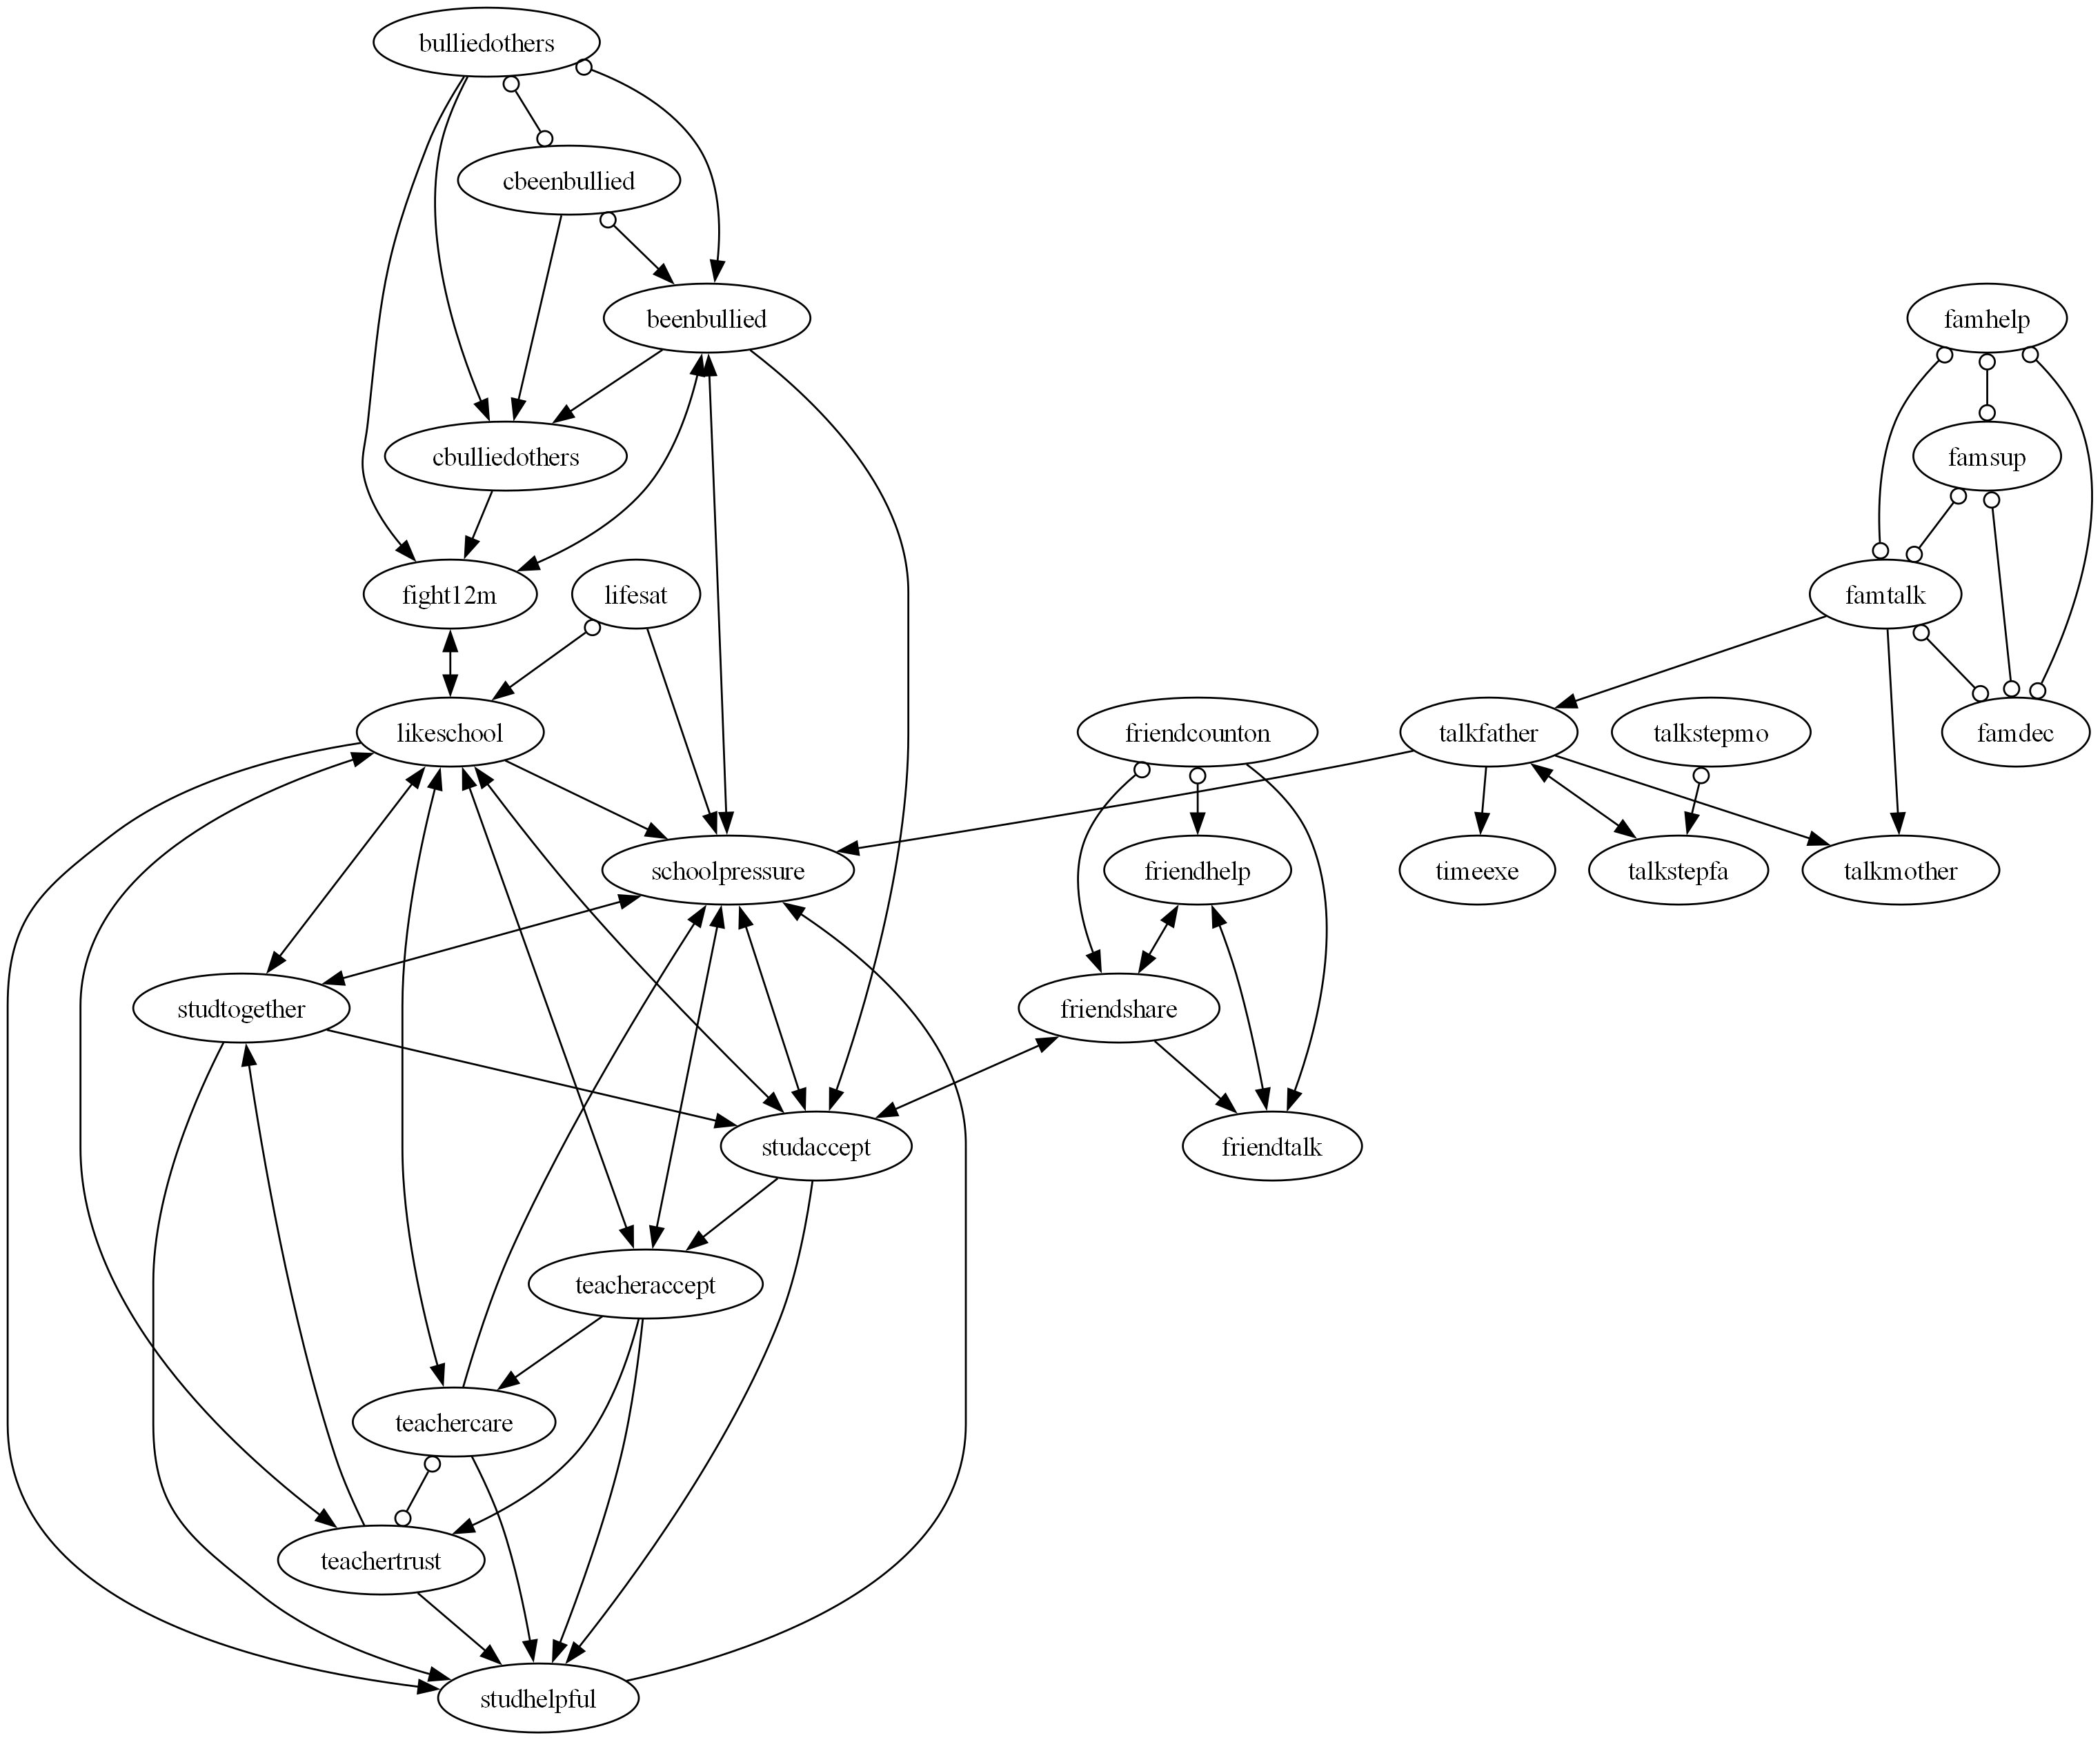
\includegraphics[width=0.8\textwidth]{Report/final_report/pictures/FCI_gsq_0.05_all_UA_27_talkmother.png}
    \caption{Findings from the FCI algorithm with $G^2$, performed at a significance level of 0.05.}
    \label{fig:fci_gsq_0.05all_UA_27_talkmother}
\end{figure}




% \begin{figure}[h]
% \centering
% \includegraphics[width=0.8\textwidth]{fci_result.png}
% \caption{Learned PAG using FCI algorithm on HBSC 2018 subset.}
% \end{figure}

\subsection{Interpretation}

The selected graph in Figure~\ref{fig:fci_gsq_0.05all_UA_27_talkmother} exhibits a modular structure, with variables organised into four thematically coherent clusters.
\subsubsection*{Bullying cluster}


\texttt{beenbullied} emerges as the central node within the bullying cluster and aligns with meta-analytic findings indicating that bullying victimisation functions both as a consequence of prior aggressive behaviours and as a catalyst for a wide range of adverse outcomes\cite{Li2024bullying}, the node directed edges from \texttt{cbeenbullied} and \texttt{bulliedothers}, with bidirected edges indicating potential latent confounding. It acts as a probable direct cause of \texttt{cbulliedothers} and \texttt{fight12m}, the latter also exhibiting a bidirected edge suggestive of an unmeasured common cause. Additionally, \texttt{studaccept} appears to be directly influenced by \texttt{beenbullied}. It might be explained by the fact that bullying victims feel unwelcome in social settings, as it adds pressure to peer-to-peer communication between students. Oftentimes, students avoid others who are being bullied for fear that they might be the next victim of bullying. A latent confounder is implied between \texttt{schoolpressure} and \texttt{beenbullied}. It could be a rival at school or a setting at school.

\texttt{bulliedothers} is directly linked to both \texttt{cbulliedothers} and \texttt{fight12m}, indicating that adolescents who bully others are likely to engage in both cyberbullying and physical aggression. Although the causal direction between \texttt{cbeenbullied}, \texttt{cbulliedothers}, and \texttt{beenbullied} is partially unresolved, the connectivity suggests a strong interplay between online and offline bullying experiences. These relations are supported by modern research. Longitudinal studies demonstrate bidirectional relationships between traditional and cyberbullying behaviours, with approximately 56\% of online bullies also engaging in face-to-face bullying\cite{Gorzig_Machackova_2015}.

\texttt{cbulliedothers} further influences \texttt{fight12m}, highlighting a potential pathway from cyberbullying perpetration to physical violence. In turn, \texttt{fight12m} affects \texttt{likeschool}, suggesting that involvement in violent behaviours negatively impacts students' school engagement\cite{Li2024bullying}.


\subsubsection*{School environment and friendship clusters}

The school environment and friendship clusters are interconnected, mirroring real-life situations where academic, peer, and friendship contexts overlap. At the centre of the school environment cluster is \texttt{studhelpful}, which is directly influenced by \texttt{teachertrust}, \texttt{teacheraccept}, \texttt{teachercare}, and \texttt{studtogether}. This suggests that helpfulness in a learning context emerges from relational dynamics with both teachers and peers. An understanding and accepting teacher might propagate their attitude to students. An edge from \texttt{likeschool} to \texttt{studhelpful} would also make sense in the opposite direction, as we would expect that students being helpful toward an individual could influence that individual's liking of school.

\texttt{teachertrust}, in particular, exhibits strong connectivity and may serve as a proxy for a safe and supportive school climate. Its bidirected edges to \texttt{teachercare} and \texttt{teacheraccept} suggest potential unmeasured common causes. These variables also feed into \texttt{studaccept}; together with \texttt{schoolpressure}, they appear to have a latent confounder. \texttt{likeschool} likely has a direct influence on \texttt{schoolpressure}. This suggests that students who feel accepted and enjoy school are less likely to experience it as a source of pressure.

The friendship cluster emerges around \texttt{friendhelp}, \texttt{friendtalk}, and \texttt{friendcounton}, with bidirected edges between them suggestive of latent variables, possibly suggesting general trust as a latent confounder. These nodes are tightly linked to \texttt{friendshare} and, through a bidirected edge, to \texttt{studaccept}, which acts  as a bridge into the academic cluster. This connection may suggest that, given a certain latent confounder, such as whether friends are schoolmates or not, positive and accepting friendships can foster peer acceptance within the school.

\subsubsection*{Parental and family communication cluster}

As expected, the family cluster is dense and tightly linked to parental support. The graph, however, represents uncertainty in causal directions within the family segment. Several connections involve edges with open circles, likely reflecting the complexity of family structures and latent variables, which may indicate a particular communication style or external, unaccounted forces that influence the family.

\texttt{famsup} appears to be the centre of the family support cluster. In real life, the feeling of being supported arises from the ability to communicate, solve problems together, and assist one another in times of need. \texttt{famtalk} serves as a bridge between the general family context and specific parental communication variables. Communication quality within a family likely acts as a direct cause of high-quality individual communication between parents and children.

Interestingly, \texttt{timeexe} has a direct edge to \texttt{talkfather}, implying that a positive relationship with one's father may encourage more physical activity or shared activities. The parental communication cluster also includes a direct edge from \texttt{talkfather} to \texttt{schoolpressure}, suggesting that good communication with one's father may reduce feelings of academic pressure, which could possibly be mediated by latent variables such as self-confidence or a sense of being supported at home.

\subsubsection*{General takeaway}
The bullying cluster, in particular, is notably intertwined with both academic and social spheres. These links back up the idea that bullying is not an isolated experience but rather a social phenomenon that occurs across both online and offline settings. The presence of bidirected edges in the cluster ( between \texttt{beenbullied} and \texttt{schoolpressure}) suggests that latent variables may underlie multiple observed associations. This may point to broader constructs such as general emotional vulnerability, peer reputation, or school climate as potential shared causes. 

\subsection{Comparison of 27-variable and 78-variable Graphs}

To examine the stability of the learned causal structure, we compared two PAGs produced by the FCI algorithm using subsets of the HBSC dataset: one with 27 variables (Figure~\ref{fig:fci_gsq_0.05all_UA_27_talkmother}) and another with 78 variables (Figure~\ref{fig:fci_gsq_0.05all_UA_78_famdec}). We aimed to assess whether the smaller graph captures core causal patterns and to what extent it can be viewed as a projection of the more complex structure.

The comparison shows a notable degree of overlap. Both graphs contain the main clusters: bullying, school engagement, peer relationships, and family communication. They share key variables such as \texttt{beenbullied}, \texttt{cbulliedothers}, \texttt{schoolpressure}, \texttt{studaccept}, and \texttt{famtalk}. Many directional edges are consistent across graphs. For instance, \texttt{cbulliedothers} $\rightarrow$ \texttt{fight12m} is preserved (with \texttt{bulliedothers} added as a mediator in the larger graph), as are \texttt{teachertrust} $\rightarrow$ \texttt{studhelpful} and \texttt{schoolpressure} $\rightarrow$ \texttt{studaccept}.

A notable difference is the reduced role of the friendship cluster. In the 27-variable graph, nodes like \texttt{friendhelp}, \texttt{friendtalk}, and \texttt{friendcounton} are tightly connected and influence school-related outcomes. In the larger graph, these nodes are present but more isolated and with undefined relations within, suggesting that peer communication becomes less central when emotional and contextual variables are taken into account.

The 78-variable graph introduces additional complexity. It includes psychosomatic symptoms (\texttt{headache}, \texttt{sleepdifficulty}), emotional indicators (\texttt{emosome01}–\texttt{emosome08}), and detailed family and socioeconomic variables (e.g., \texttt{fatherhome1}, \texttt{employfather}, \texttt{fascomputers}). These increase graph density and add new mediating paths. For example, while \texttt{lifesat} is mainly influenced by school and peers in the smaller graph, it connects to emotional and health variables in the larger one, pointing out to missing mediators in the reduced version.

Some relationships also change. In the 27-variable graph, \texttt{talkfather} directly influences \texttt{schoolpressure}. This link remains in the 78-variable graph but is now embedded within a bigger neighbourhood, including \texttt{employfather}, which may confound or mediate the relationship.

Although all 27 variables are present in the larger model, the smaller graph is not a strict subgraph. While many patterns are preserved, new edges and latent confounding structures emerge.

\subsection{Sensitivity to Parameters}

\begin{table}[hbt]
\centering
\begin{tabular}{lrrrl}
\toprule
Variables & CI test & $\alpha$ & Time (s) & Resulting graph \\
\midrule
27 & $G^2$ & 0.001 & 18 & \ref{fig:fci_gsq_0.001all_UA_27_talkmother} \\
27 & $\chi^2$ & 0.001 & 4516 & \ref{fig:fci_chisq_0.001all_UA_27_talkmother} \\
27 & $G^2$ & 0.010 & 23 & \ref{fig:fci_gsq_0.01all_UA_27_talkmother} \\
27 & $G^2$ & 0.050 & 446 & \ref{fig:fci_gsq_0.05all_UA_27_talkmother} \\
78 & $G^2$ & 0.001 & 263 & \ref{fig:fci_gsq_0.001all_UA_78_famdec} \\
78 & $G^2$ & 0.010 & 5851 & \ref{fig:fci_gsq_0.01all_UA_78_famdec} \\
78 & $G^2$ & 0.050 & 19390 & \ref{fig:fci_gsq_0.05all_UA_78_famdec} \\
\bottomrule
\end{tabular}
\caption{Summary of optimal parameters search for FCI algorithm with corresponding time required for execution. The experiments were run on 6660 records with different subsets of variables.}
\label{tab:fci_parameters_time_combined}
\end{table}



\subsubsection{Effect of Increasing \texorpdfstring{$\alpha$}{alpha}}

To investigate the sensitivity of the learned PAG structure to changes in the CI threshold, we compared graphs generated with the FCI algorithm using $\alpha$ levels of 0.001, 0.01, 0.05, and 0.1(Figures~\ref{fig:fci_gsq_0.001all_UA_27_talkmother} to ~\ref{fig:fci_gsq_0.1_for time experiment}). As $\alpha$ increases, the CI tests become more permissive, as more edges appear in the graph.

At $\alpha = 0.001$, the PAG is sparse and includes only the strongest dependencies. Many nodes appear isolated or weakly connected, especially those in the friendship or well-being domains. As $\alpha$ increases, the number of edges grows noticeably. At $\alpha=0.05$, core clusters become more densely connected, and by $\alpha=0.1$, the graph becomes highly saturated.

Across all values of $\alpha$, \texttt{schoolpressure} remains a highly connected node. As the threshold increases, it forms connections to variables such as \texttt{beenbullied}, \texttt{lifesat}, and \texttt{talkfather}, which bridge between academic stress, social dynamics, and family communication.

 The number of bidirected edges, or identified latent confounding patterns, increases with $\alpha$. Notably, these appear among variables such as \texttt{teachertrust} and \texttt{teachercare}, or \texttt{beenbullied} and \texttt{schoolpressure}. 

At lower $\alpha$ values, the family communication variables are mostly self-contained and have no causal directions. As $\alpha$ increases, variables like \texttt{talkfather} begin to connect with school-related outcomes, including \texttt{schoolpressure} and \texttt{lifesat}. 

Increasing $\alpha$ in the FCI algorithm results in denser graphs with more discovered edges and a higher prevalence of latent confounding structures. The graph at $\alpha = 0.05$ appears to show a balance between interpretability and coverage relations within data. It maintains the clustering while capturing meaningful dependencies. Lower $\alpha$ values yield cleaner, more conservative graphs suitable for high-confidence interpretations, while higher $\alpha$ values expose richer and more exploratory causal pathways. However, despite the benefits of causal graphs, they should be carefully reviewed and interpreted in conjunction with background knowledge and alternative research.



\subsubsection{CI test role}
To isolate the effect of the CI test used, we compared two PAGs estimated at the same significance level $\alpha = 0.001$: one using the $G^2$ test (Figure~\ref{fig:fci_gsq_0.001all_UA_27_talkmother}) and the other using the $\chi^2$ test (Figure~\ref{fig:fci_chisq_0.001all_UA_27_talkmother}).

The graph based on the $\chi^2$ test is significantly denser than the one based on $G^2$, with more directed and bidirected edges across clusters, higher connectivity, and more inferred causal and confounding relationships.

In the $\chi^2$ graph, the friendship cluster (\texttt{friendhelp}, \texttt{friendcounton}, \texttt{friendshare}, \texttt{friendtalk}) is tightly connected and links to broader constructs such as \texttt{lifesat}, \texttt{famsup}, and \texttt{schoolpressure}. The family communication variables are also more integrated, while they form edges with both school-related and emotional variables. In contrast, the $G^2$ graph presents these clusters as disconnected, with \texttt{lifesat} entirely disconnected and minimal influence from peer or family support pathways.

Both graphs preserve the core components of the school and bullying clusters. However, the $G^2$ graph shows a more detailed picture: for example, \texttt{beenbullied} connects to both \texttt{schoolpressure} and \texttt{lifesat}. Additionally, the $\chi^2$ graph includes bidirected edges between \texttt{cbulliedothers} and \texttt{cbeenbullied}, as well as between schoolpressure and friendshare, indicating latent confounding. Such patterns are mainly absent in the $G^2$ graph, where the bullying variables remain internally clustered with undefined paths but disconnected from other domains.

\end{document}